\documentclass[fontset=none]{ctexart}

\usepackage[T1]{fontenc}
\usepackage{fontspec}
\setCJKmainfont{SimSun}
% Latin Modern
\renewcommand*\ttdefault{txtt} % 改等宽字体

\setcounter{tocdepth}{5}
\setcounter{secnumdepth}{5}
% -1 part
% 0 chapter
% 1 section
% 2 subsection
% 3 subsubsection
% 4 paragraph
% 5 subparagraph

\usepackage{cite}
\usepackage{geometry}
\geometry{a4paper,scale=0.7}

\usepackage{algorithm}  
\usepackage{algorithmicx}  
\usepackage{algpseudocode}
\makeatletter
\newenvironment{breakablealgorithm}
  {% \begin{breakablealgorithm}
   \begin{center}
     \refstepcounter{algorithm}% New algorithm
     \hrule height.8pt depth0pt \kern2pt% \@fs@pre for \@fs@ruled
     \renewcommand{\caption}[2][\relax]{% Make a new \caption
       {\raggedright\textbf{\ALG@name~\thealgorithm} ##2\par}%
       \ifx\relax##1\relax % #1 is \relax
         \addcontentsline{loa}{algorithm}{\protect\numberline{\thealgorithm}##2}%
       \else % #1 is not \relax
         \addcontentsline{loa}{algorithm}{\protect\numberline{\thealgorithm}##1}%
       \fi
       \kern2pt\hrule\kern2pt
     }
  }{% \end{breakablealgorithm}
     \kern2pt\hrule\relax% \@fs@post for \@fs@ruled
   \end{center}
  }
\makeatother

\usepackage{amsmath}
\usepackage{amssymb}
\usepackage{graphicx}
\usepackage{subfigure}
\usepackage{changepage}
\usepackage{multirow}
\usepackage{url}

\usepackage{amsthm}
\newtheorem{theorem}{Theorem}[section]
\newtheorem{lemma}[theorem]{Lemma}
\newtheorem{proposition}[theorem]{Proposition}
\newtheorem{corollary}[theorem]{Corollary}
% \newtheorem{remark}{Remark}[section]
\newtheorem{example}{Example}[section]
\newenvironment{solution}{\begin{proof}[Solution]}{\end{proof}}
\theoremstyle{definition}
\newtheorem{definition}{Definition}[section]
\theoremstyle{remark}
\newtheorem*{remark}{Remark}

\usepackage[colorlinks, linkcolor=black, citecolor=blue, bookmarksnumbered]{hyperref}
% \hypersetup{
% 	colorlinks=true,
% 	linkcolor=cyan,
% 	filecolor=blue,      
% 	urlcolor=red,
% 	citecolor=green,
% }

\usepackage{fancyhdr}
\pagestyle{fancy}
\renewcommand{\sectionmark}[1]{\markright{\thesection\ #1}}
\fancyhf{}
\cfoot{\thepage}
\lhead{\rightmark}
% \rightmark 当前的节名
% \leftmark 当前的章名
% \(l/c/r)head{}, \(l/c/r)foot{}
\renewcommand{\headrulewidth}{0.4pt}
\renewcommand{\footrulewidth}{0pt}

\renewcommand\refname{References}
\renewcommand\contentsname{Content}
\renewcommand\figurename{Figure}

\begin{document}

\begin{titlepage}
    \begin{center}
        \vspace*{1cm}
            
        \Huge
        \textbf{Design and Implementation of A TTE System}
            
        \vspace{0.5cm}
        \LARGE
        Second Report\\
            
        \vspace{1.5cm}
            
        \textbf{11812804}  董\quad 正\\
        \textbf{11813225}  王宇辰\\
        \textbf{11811305}  崔俞崧\\

        \vspace{0.5cm}
        Supervisior: 宋轩
            
        \vfill
            
        
\includegraphics[width=\textwidth]{images/sustc.png}
            
        \vspace{0.2cm}
            
        \Large
        Department of Computer Science and Engineering\\
        \vspace{0.5cm}
        May. 2021
            
    \end{center}
\end{titlepage}

\tableofcontents

\clearpage
\section{Preliminaries}
\subsection{Review}
\subsubsection{TTE}
\textbf{Travel Time Estimation (TTE)} is one of the most important researching topic in the traffic forecasting field. 
Estimating the travel time of any path in a city is of great importance to traffic monitoring, route planning, ridesharing, taxi dispatching, etc.
On Sep. 2020, DeepMind published a blog named \textit{Traffic prediction with advanced Graph Neural Networks}. 
This blog briefly described the whole industrial structure of estimated times of arrival (ETAs) techniques applied in Google Map but did not given any detailed implementation or any code.
Our work is based on the model structure of TTE proposed in the blog.
\begin{figure}[htb]
    \centering
    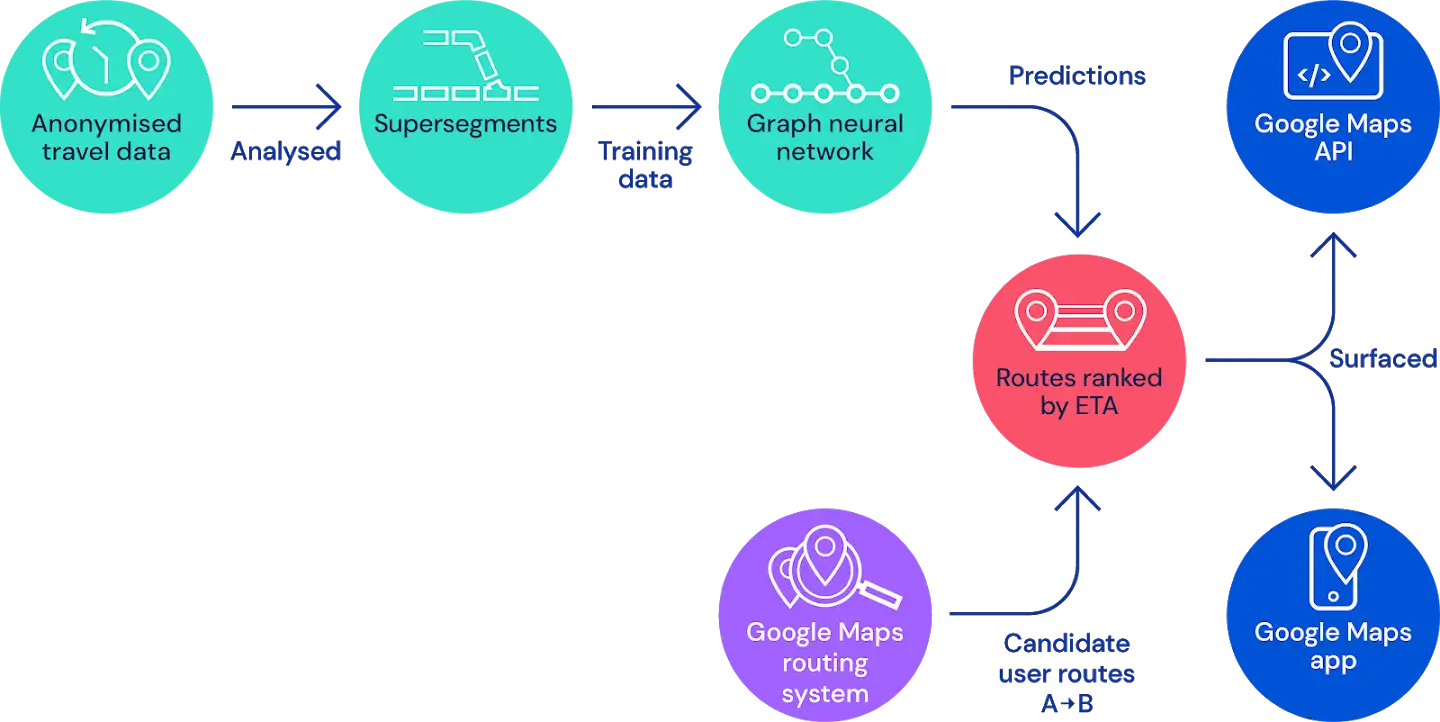
\includegraphics[width=0.9\textwidth]{images/architecture.png}
    \caption{Architecture}
    \label{fig1}
\end{figure}

\subsubsection{Goal}
Our ultimate goal (tentative) is to implement the industrial structure and apply it to the open source databases in China, then compare the performance with the state-of-the-art structures and find its application value.
This semester, we will implement a TTE system base on the work we done in the last term, combining \textit{Supersegment} and TTI.
We will try to work out an interactive application with graphical user interface. 

\subsection{Introduction}
In last stage, we finished the code of \textit{Supersegment} and made a simple UI design of our application.

Breifly, we will state our work in this report as
\begin{itemize}
  \item TTE Web APP Design by 董正 \& 王宇辰
  \item Computing TTI by 崔俞崧
\end{itemize}

\clearpage
\section{TTE Web APP Design}


\clearpage
\section{Computing TTI}

% \clearpage
% \phantomsection
% \addcontentsline{toc}{section}{References}
% \bibliographystyle{ieeetr}
% \bibliography{references}

\end{document}